
\section*{The Universe}
In the beginning the Universe was created. This has made a lot of people very angry and been widely regarded as a bad move.
I know why everybody is this angry about it, but it really just sounds like their problem.

In figure \ref{fig:universe} you can see a picture of a galaxy.

\begin{figure}[h]
  \center
  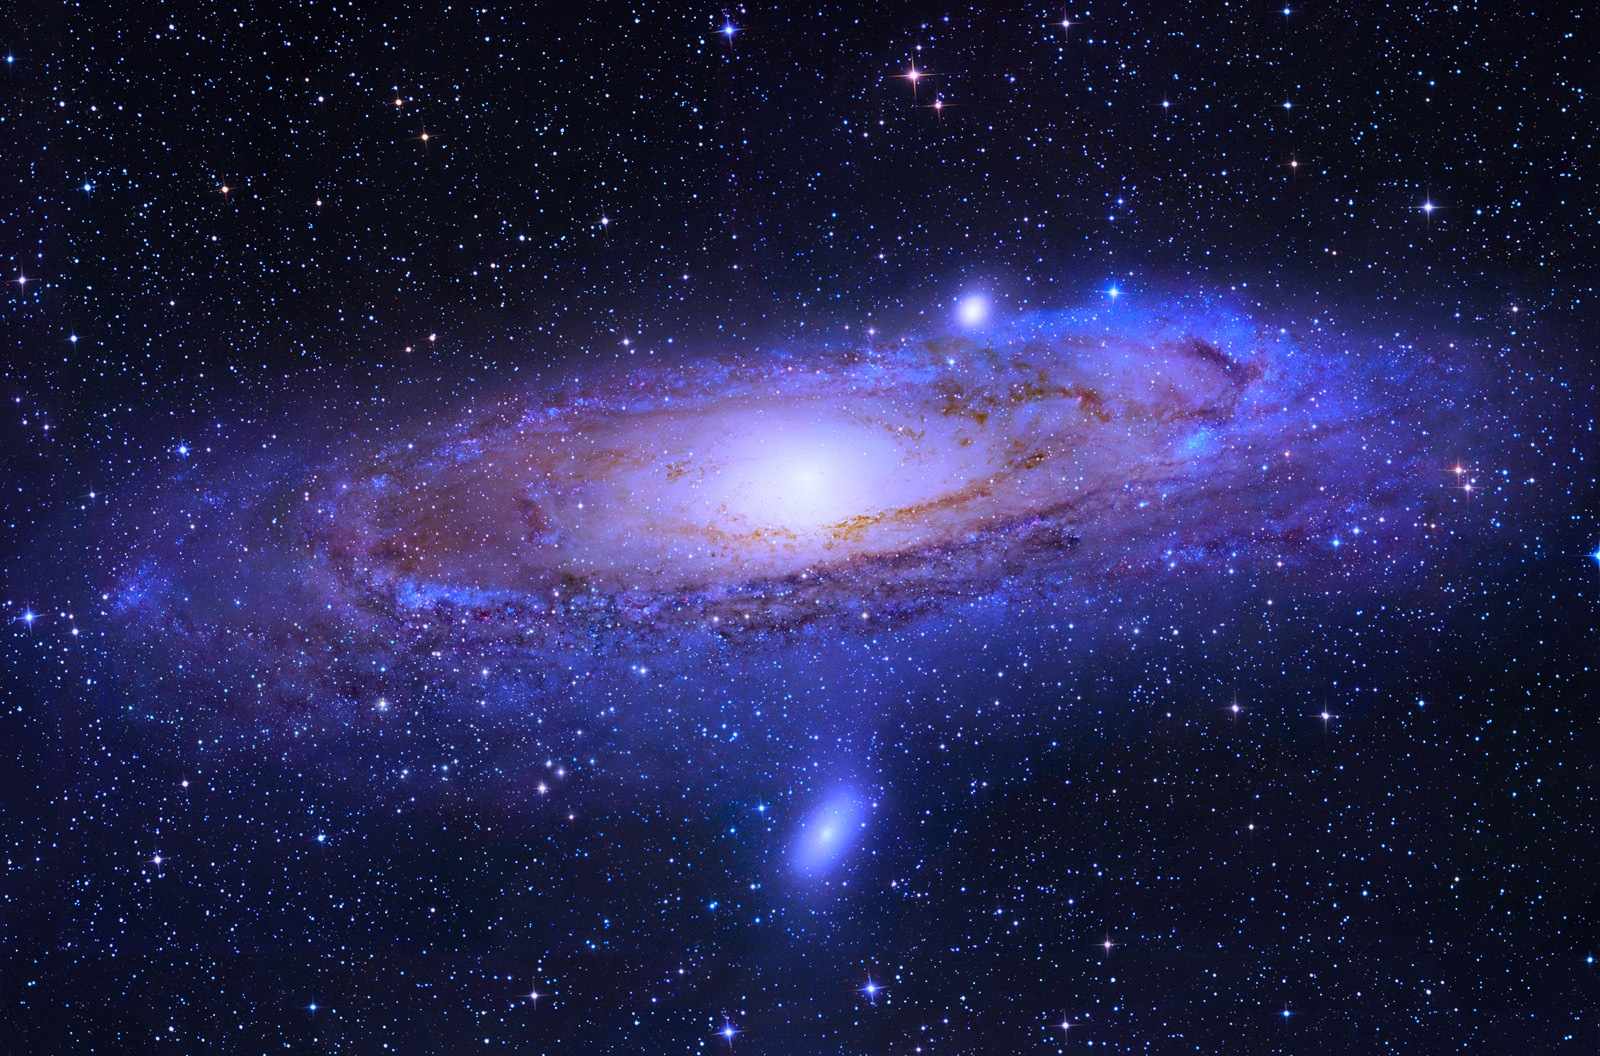
\includegraphics[width=0.6\textwidth]{galaxy.jpg}
  \caption{A picture of a galaxy}
  \label{fig:universe}
\end{figure}

A galaxy is really big. You're just a tiny spec of dust in comparison. Now, there are a lot of galaxies in the universe.
So many indeed, that there are galaxy clusters, where multiple galaxies are grouped together based on the distance between them.
But that's not enough yet. There are also clusters of clusters. And then there's groups of clusters.

The universe is really big. We don't even really know how big. Why? We can't even see it's borders, because light from there hasn't reached us yet.

In a believed stroke of genius, some may say that there's still something more massive, your mom. However, since we're here to proof that you're insignificant,
your mom can't be this massive, or it would be something you'd be significant for.